\chapter{Theoretical Background}
As seen in the related work section, many sophisticated ideas have already been proposed stating how the task of motion segmentation on RGB-D videos can be addressed. In this thesis, we aim to approach this issue by incorporating optical flow fields to track motion trajectories and then group them by running a spectral clustering. However, there exist many possibilities how to implement a spectral clustering on trajectories. \\ \\
In this chapter we give an introduction about various mathematical concepts which form the fundament to understand the implementation of our motion segmentation pipeline and how its results were computed. In particular, we will discuss the concepts of optical flow and spectral clustering, since they are essential concepts used throughout this thesis. \\ \\
We start by defining a general motion segmentation pipeline and elaborate on its stages, which later will be used as a blue print for our later pipeline implementation. Next we give a brief introduction in optical flow fields by offering the reader a basic definition, some insights about the pioneering motion estimation work of Horn and Schunck and summarize four modern flow methods. We will see that optical flow fields are particularly useful for tracking point trajectories. Since we determine motion by grouping trajectories, the quality of the optical flow affects the final outcome of the motion segmentation. \\ \\
Finally, since our pipeline implements segmentation methods that are all based on spectral clustering variants, we wrote a dedicated section about clustering data points, in which we explain the idea behind clustering methods and how they can be implemented. Moreover, we state some important definitions about similarity graphs and their properties, how to form the Laplacian matrix from a similarity graphs and the differences between k-means and spectral clustering. We conclude this section by stating that optimizing for the minimum cut on a similarity graph is an equivalent to the problem of computing the spectral clustering on its Laplacian matrix. 

\section{General Motion Segmentation Pipeline}
In this section, we conceptually describe how the task of motion segmentation can be approached. As mentioned earlier, motion segmentation is the task of decomposing a video sequence into its moving objects and into its background. The idea is to separate image regions that undergo different motion patterns. Therefore, we want to consider motion not independently for each frame but rather the whole history of a point to make a grouping decision. The history of a point can be represented by point trajectories which are the result of a point tracker. The point tracking is based on optical flow fields. \\ \\
Since point trajectories have a temporal- (via the frames the capture) as well as a spatial (via image location in captured frames via the tracked points) component, they are an ideal intermediate representation for the motion of object parts. \\ \\
In recent Computer Vision literature, various contributions have already successfully demonstrated that motion segmentations can be cast as the problem of clustering point trajectories from an image sequence with respect to their motion. For instance in $\cite{OB14b}$, T.Brox et al implemented a motion segmentation based on a spectral clustering on motion trajectories. In particular, they described a certain similarity measure that can be used to form such a similarity matrix. In $\cite{KB15b}$ the authors followed a similar approach but formed a similarity graph. The segmentation was generated by running a multi min-cut. \\ \\
In this thesis we want to follow a similar approach as described in those two contribution. For this purpose we compared their segmentation pipelines and derived a general motion segmentation pipeline. In summary, a motion segmentation pipeline implements the following main stages:
\begin{enumerate}
	\item Compute optical flow fields on the video sequence.
	\item Extract meaningful motion feature locations in the video frames.
	\item Track motion trajectories on feature locations using the flow fields.
	\item Compute affinities between these trajectories and form a similarity matrix.
	\item Group the trajectories via a spectral clustering on the affinity matrix.
\end{enumerate}
However, keep in mind that this motion segmentation technique also suffers from some issues: Trajectories usually start and end in different frames due to occlusion and disocclusion. Therefore, it is crucial to know where points get occluded. Furthermore, there are various metrics that can be used to compute distances between trajectories, such as their spatial-, color- or motion-distance. Moreover, there are many mathematical variants to solve the problem of spectral clustering. Lastly, the used optical flow estimation method should be carefully chosen since it affects the quality of the final segmentation. \\ \\
In next chapter we describe how we implemented such a motion segmentation pipeline by following these main stages. In particular, we will address all issues described above and provide robust solutions.

\section{Optical Flow}
\label{sec:optical_flow}
In this section we, explain the principles and the idea behind optical flow. We motivate this concept by discussing an intuitive example, followed by stating a mathematical definition. Furthermore, we explain how such a flow field could be visually represented. Lastly, we summarize and elaborate on the pioneering formulation of Horn and Schnunck, which can be used to estimate flow fields.

\subsection{Motivation}
The optical flow ($\textbf{OF}$) is a vector field that defines a point-to-point correspondence between two successive frames. Each vector acts as the displacement of a point in the first frame to match its corresponding point in the second frame. In other words, the OF represents the pixel motion field as observed in images and thus answers the question which pixel went where in its successor frame. Ideally, the optical flow is the projection of the three dimensional motion on an image. \\ \\
Figure $\ref{fig:optical_flow_math_def_eg}$ illustrates the idea of the point-to-point correspondence using optical flow fields.
\begin{figure}[H]
\begin{center}
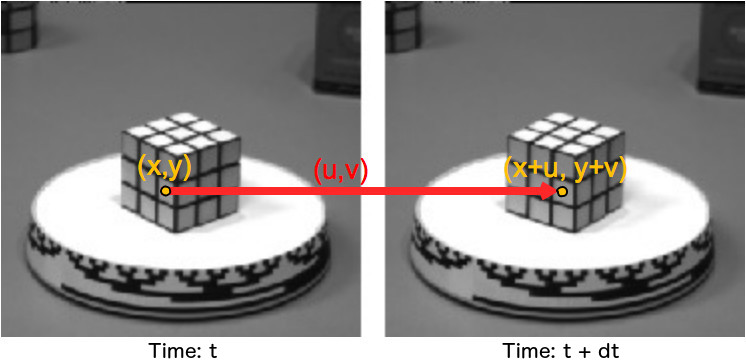
\includegraphics[width=1\linewidth] {background/of/rubiks_cube_frames}
\end{center}
\caption[Spinning Rubik's Cube]{An illustration$\footnotemark$ of two frames of a spinning Rubik's Cube. The point-to-point correspondence of a sample point (the orange point) is given by the optical flow, depicted as a red arrow.}
\label{fig:optical_flow_math_def_eg}
\end{figure}
\footnotetext{The unprocessed image shown in this figure has been taken from: \\ \url{http://robotics.eecs.berkeley.edu/~sastry/ee20/vision3/node2.html}}
In this figure two frames of a spinning Rubik's cube at different times are shown. The orange point $p = (x,y)$ at time $t$ is tracked to the position $(x+u, y+v)$ at time $t+dt$ by adding the optical flow $(u,v)$ (visualized by a red arrow) to $p$. This matter of a fact can mathematically be modelled via the brightness consistency assumption, stated in Equation $\ref{eq:of_brightness_const}$.
\begin{equation}
	I_{t} \left( x,y \right) = I_{t+dt} \left( x+u, y+v \right)
\label{eq:of_brightness_const}
\end{equation}
Where $I_t$ depicts the brightness at frame $t$.

\subsection{Visualization of Flow Fields}
For visualizing flow fields we use the Middlebury$\cite{Baker2011}$ flow color encoding$\footnote{The corresponding visualizer script can be found at \url{http://vision.middlebury.edu/flow/submit/}}$ shown in Subfigure $\ref{fig:color_encoding_flows_a}$. The shown color plate provides color values for the normalized$\footnote{One way to normalize a set of vectors is the following: Divide each vector by the maximal length of these vectors.}$ flow vectors. The angle in the circle corresponds to the flow direction and the distance to the center corresponds to the flow velocity. Moreover, Figure $\ref{fig:color_encoding_flows}$ also contains an example of a flow visualization using these color codes. As we can see the cars are moving to the bottom-right direction at a intermediate velocity.
\begin{figure}[H]
\begin{center}
\subfigure[Flow Color Codes]{
   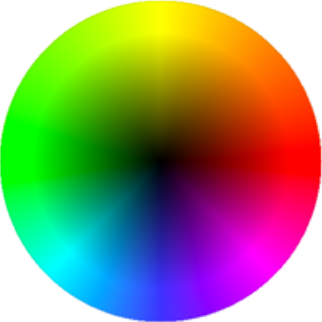
\includegraphics[width=0.40\linewidth] {background/of/flowfield_color_encoding}
   \label{fig:color_encoding_flows_a}
}
~
\subfigure[Example flow visualization]{
   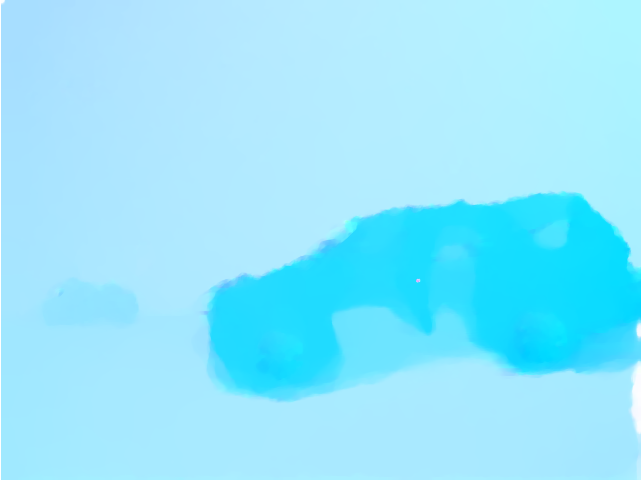
\includegraphics[width=0.535\linewidth] {background/of/cars_fwf_1}
   \label{fig:color_encoding_flows_b}
}
\end{center}
\caption[Visual Color Encoding of Flow Fields]{On the left a visualization of the color plate used to draw flow fields and on the right flow field visualized by this color scheme.}
\label{fig:color_encoding_flows}
\end{figure}

\subsection{Original Flow Estimation Method of H.S.}
\label{sec:hs_formulation}
In the pioneering work of $\cite{Hs81}$, B. Horn and B. Schnunck describe a technique to estimate the optical flow. Their method assumes smoothness in the flow over the whole image. Their flow estimation is formulated as a global energy functional and can numerically be solved via the Jocobi method$\footnote{The Jacobi method is an iterative method used to solve linear systems.}$. The advantage of their method is that it produces flow fields where the inner parts of homogeneous objects is filled in from the motion boundaries. However, its downside is that is very sensitive to noise. \\ \\
Back then they defined the optical flow as \textit{the distribution of apparent velocities of movement of brightness patterns in an image}. \\ \\
Moreover, they already understood the potential of the optical flow and stated the following properties: It can arise from relative motion between objects and the viewer, provides information about the spatial arrangement of the viewed objects and the rate of change in that arrangement. Moreover, they mentioned that discontinuities in the optical flow can help to perform segmentation tasks. \\ \\
Sticking to their flow definition they derived an equation that relates the change in the image brightness at a point to the motion of the brightness. \\ \\
Their formulation is based on the following assumptions:
\begin{itemize}
  \item The surface is assumed to be flat. This avoids brightness variations due to shading effects.
  \item The incident illumination is uniform across the surface. Then, the brightness at a point in the image is proportional to the reflectance of the surface at the corresponding point on the object.
  \item The Reflectance varies smoothly and has no spatial discontinuities. Having no discontinuities assures that the image brightness is differentiable.
  \item Situations where objects occlude one another are excluded.
\end{itemize}
These assumptions allow to conclude, that in their model the brightness of a particular point in the pattern is constant. \\ \\
Let the image brightness at a point $(x,y)$ in the image plane at time $t$ be denoted by $E(x,y,t)$. Since the brightness of any point is constant, the total derivative $\frac{d E}{dt}$ is zero. Using the chain rule for differentiation, they derived the expression in Equation $\ref{eq:flow_eq}$.  
\begin{equation}
\begin{aligned}
0 &= \frac{d E}{dt} \\
&= \frac{\partial E}{\partial x} \frac{x}{dt} + \frac{\partial E}{\partial y} \frac{y}{dt} + \frac{\partial E}{\partial t} \\
&= E_{x} u + E_{y} v + E_{t}
\end{aligned}
\label{eq:flow_eq}	
\end{equation}
where we the following substitutions were used to derive the last identity of Equation $\ref{eq:flow_eq}$:
\begin{equation}
\begin{aligned}
	u = \frac{dx}{dt} \text{ and } v = \frac{dy}{dt}
\end{aligned}
\end{equation}
By re-ordering the terms of Equation $\ref{eq:flow_eq}$ the same way like it has been done in Equation $\ref{eq:reordered_flow_eq}$:
\begin{equation}
\begin{aligned}
	(E_x, E_y) \cdot (u, v) &= -E_t \\
	\underbrace{-\frac{1}{E_t}\left( E_x, E_y \right)}_\text{known} \cdot \underbrace{(u, v)}_\text{unknown} &= 1
\end{aligned}
\label{eq:reordered_flow_eq}
\end{equation}
Hence, they could show that the change in image brightness can be formulated by a single linear equations with two unknowns $u$ and $v$, the so called $\textit{flow velocity}$. As a consequence, such a flow velocity cannot be computed locally without introducing additional constraints. \\ \\
In their formulation they express their additional constraint by stating that the square of the magnitude of the gradient of the optical flow velocity, as defined in Equation $\ref{eq:smoothness_constraints}$
\begin{equation}
	\left( \frac{\partial u}{\partial x} \right)^2 + \left( \frac{\partial u}{\partial y} \right)^2 \text{ and } \left( \frac{\partial v}{\partial x} \right)^2 + \left( \frac{\partial v}{\partial y} \right)^2,
\label{eq:smoothness_constraints}
\end{equation}
should be minimal. The remaining problem is then to minimize the sum of the energies modelling the rate of image brightness change as stated in Equation $\ref{eq:energy_brightness}$
\begin{equation}
	E_b = E_x u + E_y v + E_t
\label{eq:energy_brightness}
\end{equation}
and the measure of the departure from smoothness in the velocity flow, as formulated in Equation $\ref{eq:energy_constraint}$.
\begin{equation}
	E_c^2 = \norm{\nabla u}^2 + \norm{\nabla v}^2
\label{eq:energy_constraint}
\end{equation}
The total error to be minimized is therefore equal to the energy term formulated in Equation $\ref{eq:final_hs_energy_term}$.
\begin{equation}
	E = \int \int \left( E_b^2 + \alpha^2 E_c^2 \right) dx dy
\label{eq:final_hs_energy_term}
\end{equation}
This flow estimation formulation assumes smoothness in the flow over the whole image. Hence, minimzing this energy results in a minimization of distortions in the flow and thus prefers solutions which exhibit more smoothness. The scalar $\alpha$ acts as a regularization constant, that weights the influence of the smoothness term. Hence, larger values for $\alpha$ lead to soother flow estimations. \\ \\
This minimization can analytically be solved by formulating its multi-dimensional Euler-Lagrange equations as formulated in Equation $\ref{eq:multi_dim_euler_lagrange}$.
\begin{equation}
\begin{aligned}
 \frac{\partial L}{\partial u} - \frac{\partial}{\partial x} \frac{\partial L}{\partial u_x} - \frac{\partial}{\partial y}\frac{\partial L}{\partial u_y} &= 0 \\
\frac{\partial L}{\partial v} - \frac{\partial}{\partial x} \frac{\partial L}{\partial v_x} - \frac{\partial}{\partial y}\frac{\partial L}{\partial v_y} &= 0  
\end{aligned}
\label{eq:multi_dim_euler_lagrange}
\end{equation}
where L denotes the integrand of the energy expression, given by Equation $\ref{eq:def_l_euler_lag}$:
\begin{equation}
\begin{aligned}
E_x E_b - \alpha^2 \Delta u &= 0 \\
E_y E_b - \alpha^2 \Delta v &= 0 \\
\end{aligned}
\label{eq:def_l_euler_lag}
\end{equation}
Where $\Delta$ denotes the Laplace$\footnote{Definition of the Laplace operator in the two dimensional case: $\Delta = \frac{\partial^2}{\partial x^2} + \frac{\partial^2}{\partial y^2}$}$ operator. When using a finite differences scheme for approximating the Laplacian equation
as defined in Equation $\ref{eq:finite_difference_laplacian}$
\begin{equation}
	\Delta u(x,y) = \bar{u} (x,y) - u(x,y)
\label{eq:finite_difference_laplacian}
\end{equation}
where $\bar{u} (x,y)$ denotes the weighted average of u computed by visiting the neighborhood around the pixel at location $(x,y)$, Equation $\ref{eq:def_l_euler_lag}$ can be simplified to
\begin{equation}
\begin{aligned}
(E_x^2 + \alpha^2) u + E_x E_y v &= \alpha^2 \bar{u} - E_x E_t \\
(E_x^2 + \alpha^2) v + E_x E_y u &= \alpha^2 \bar{v} - E_y E_t
\end{aligned}
\label{eq:def_l_euler_lag_simplified}
\end{equation}
The equations from above (Eq. $\ref{eq:def_l_euler_lag_simplified}$) became linear in $u$ and $v$. This allows to solve this minimization problem for each pixel in the image. However, keep in mind that the solution depends on the neighboring values of the flow field. Hence, the system must be solved iteratively. The following update rule can therefore be used:
\begin{equation}
\begin{aligned}
 u_{k+1} &= \bar{u}_k - \frac{E_x (E_x \bar{u}_k + E_y \bar{v}_k + E_t)}{\alpha^2 + E_x^2 + E_y^2} \\
  v_{k+1} &= \bar{v}_k - \frac{E_y (E_x \bar{u}_k + E_y \bar{v}_k + E_t)}{\alpha^2 + E_x^2 + E_y^2}
\end{aligned}
\label{eq:hs_iteration}
\end{equation}

\subsection{Modern Flow Methods}
\label{sec:impl_optical_flow}
In this section we briefly summarize four modern flow methods. Additionally, we state their main properties and their drawbacks. Discussing those methods particularly makes sense since we make use of these flow estimation techniques later in our pipeline to generate flow fields.

\subsubsection{Enhanced H.S. Optical Flow Fields}
In $\cite{Deq10}$ Dequing Sun et al studied various flow methods and models and determined the most important factors that increase the quality of produced flow fields. They incorporated their findings in Horn and Schunck's original formulation and contributed a efficient implementation of their method. Additional information about their formulations can be found in Section $\ref{sec:hs_formulation}$ on page $\pageref{sec:hs_formulation}$. \\ \\
When using the abbreviation HS we strictly refer to their implementation. \\ \\
The original HS formulation combines a data term that assumes constancy of some image property with a spatial term that models how the flow is expected to vary across the image. The HS model relies on brightness constancy and spatial smoothness assumptions. Unfortunately it is not very robust to outliers. Therefore, the following main improvements were implemented in their methods:
\begin{itemize}
  \item The quadratic penalty function is replaced by the Charbonnier penalty $p\left( x \right) = \sqrt{x^2 + \epsilon^2}$. This penalty is supposed to be less error-prone to outliers.
  \item An incremental multi-resolution technique is applied to estimate flow fields with large displacements. The optical flow estimated at a coarse level is used to warp the second image toward the first at the next finer level and a flow increment is calculated between the first image and the warped second image. Each level is recursively downsampled by applying a Gaussian filter from its nearest lower level.
  \item An enhanced objective function is used, which includes a non-local term that robustly integrates flow estimates over large spatial neighborhoods. This is achieved by applying a median filtering to denoise the flow after every warping step to increase the accuracy.
\end{itemize}

\subsubsection{Large Displacement Optical Flows}
Before the work in $\cite{Bro11a}$, there was no accurate method present to estimate fast motions of small objects, i.e. large motions. Most flow methods are based on a combination of HS flow formulation and the concept of coarse-to-fine image warping. However, both approaches have been extended by robust statistics to fight outliers and the same time retain smoothness assumptions. \\ \\
Two fundamental ideas exist to address the issue of large motions. On on hand there are coarse-to-fine techniques. Such techniques, however, require a downsampling. Unfortunately, this also removes details that may be important for the flow accuracy. consequently, the method cannot refine the flow of structures that are smaller than their displacement, because the structure is smoothed away. Flow Fields produced this way are often close to the motion of the larger scale structures. \\ \\
On the other hand descriptor matching techniques are well suited to match large displacements. However, their resulting correspondences are very sparse, have limited accuracy and exhibit many outliers to to missing regularity constraints and lastly, there is only pixel-level accuracy. \\ \\
In their paper they propose a method how to combine both strategies. They direct a variational technique using correspondences from sparse descriptor matching. The correspondences determined by the descriptors are directly integrated into the variational approach. The allows to make use of all image information at every level and smoothly scales down the influence of descriptor keypoints as the grid gets finer.

\subsubsection{Semi Rigid Scene Flows}
In their paper $\cite{Bro14}$, Quiroga et al. proposed an approach to estimate the scene flow$\footnote{The term scene flow denotes a motion field in the 3d space, which can be computed from a single view when using RGB-D sensor data.}$ by exploiting the properties of motion in real world scenes. For that purpose they implemented an over-parameterized framework that estimates scene flows from RGBD images. \\ \\
This allows for piecewise smooth solutions using a total variation (TV) regularization$\footnote{An image denoising technique, which is also known as \textit{total variation denoising}.}$ on the parameterization. Most real world scenes can be modelled as locally or piecewise rigid. This means that the scene is composed of 3d independently rigid components. Moreover, their formulation offers a general formulation to solve for the local and global motion by jointly using intensity and depth data. \\ \\
They model the scene flow as a 3d vector field consisting of a global rigid motion plus a non-rigid residual. this is particularly useful, when estimating the motion of deformable objects in conjunction with a moving camera. A piecewise smooth solution is estimated using a total variation on the parameterization.\\ \\
In the following some details according to their implementation:
\begin{itemize}
  \item They represent motions as a 3d vector field of twists, which encourages piecewise-smooth solutions of rigid body motions.
  \item Instead of representing the flow vectors in the 3d space, they represent the scene structure in the image domain. Then, color and depth data can be coupled using a projective function. this way depth influences the motion in the image domain and consistency constraints can be formulated jointly over the color and depth images. 
  \item However, scene flow estimation using intensity and depth is an ill-posed problem and regularization is needed. In their work they use an over-parameterization of the scene flow. Each scene point is allowed to follow a rigid body motion. this way, the regularization can be done on a field of rigid motion.
  \item Usually, the 3d motion vector of each point is solved to minimize color and intensity constraints in a data term and the whole 3d motion field is regularized to get spatially smooth solutions while preserving discontinuities. Since depth data is available a weighted regularization can be used to preserve motion discontinuities along depth edges. 
  \item In order to formulate an efficient 3d motion exploration they use a parameterization provided by RGB-D sensors to formulate an efficient 3d motion exploration. Hence, they define a warping function to couple the twist motion and the optical flow. They use a warping function to locally constrain the rigid motion field in the image domain and define a depth consistency constraint to exploit the sensor data.
\end{itemize}

\subsubsection{Layered RGB-D Flow Fields}
%s1
%estimate general 2D motion by decomposition into several layers, which enables occlusion reasoning
%s2
%Other methods do segment the scene to impose rigidity or strong regularization over the regions (or segments). However, these segmentations are only used as tools to improve the accuracy of the estimates, and do not really cor-
%respond to the underlying/independent motions of the scene => partitions the scene into depth layers
In $\cite{Deq10}$ Dequing Sun et al present a layered RGBD scene flow estimation  method. They make use of the fact that depth information allows to recover 3d motion from a single view. However, in that case, depth boundaries are not well aligned with RGB images. Especially in occluded regions methods produce large errors. As a remedy, they therefore, use the depth fields for occlusion reasoning and formulate a layered RGBD scene flow method that jointly solves for the scene segmentation and the motion. In their formulation, the depth fields are used to estimate the per-layer 3d rigid motion to constraint the motion of each layer. \\ \\
The implementation of their method is freely available on the authors website, written in Matlab. In the following we use the abbreviation LRGBD for flow fields produced by their implementation. \\ \\


\section{On Data Clustering}
\label{sec:on_data_clustering}
Clustering is a technique for exploratory data analysis and allows to identify groups of similar behaviour. This is achieved by separating data points according to their similarities. \\ \\
Generally, clustering is a hard problem and yet no perfect method exists. As we show in our evaluation section, the choice of the segmentation method has a big influence on the quality of our motion segmentation pipeline. \\ \\
In this section we offer the reader definitions of various such techniques. For writing the content of this section we partially relied on the work of $\cite{vonLuxburg2007}$. \\ \\
In the following we start by describing the k-means clustering which is a clustering method applied on point clouds and which is popular because of its speed, relative simplicity and robustness. However, a drawback of k-means is that it only works for relatively low-dimensional datasets. \\ \\ 
In this thesis, we are mainly working with datasets consisting of point trajectories. This kind of data is not easily embeddable in an Euclidean space. Therefore, we present a more general clustering framework targeting at segmenting graphs. Regardless of the dimensionality of the input data, these method are general enough to work with any kind of data as long as it is possible to compute a distance between data point pairs

\subsection{K-Means Clustering}
\label{sec:k_means}
The idea of the k-means clustering algorithm is to partition $n$ observations into $k$ clusters in which each observation belongs to the cluster with the nearest mean. \\ \\
Given a set of observations $(\textbf{x}_1, \dots, \textbf{x}_n)$, where any $\textbf{x}_k \in \mathbb{R}^d$. k-means clustering tries to partition the $n$ observations into $k$ sets $\textbf{S} = \{ S_1, \dots, S_k\}$ to minimize the sum of distance functions of each point in the cluster to the $k$ centers. Mathematically, this can formulated as follows:
\begin{equation}
	\argmin_{\textbf{S}} \sum_{i=1}^k \sum_{\textbf{x} \in S_i} \norm{\textbf{x} - {\boldsymbol {\mu }}_{i}}^2
\label{eq:k_means_minimzation_formulation}
\end{equation}
where ${\boldsymbol {\mu }}_{i}$ is the mean of points in $S_i$, the so called centroid. \\ \\
The k-means clustering equations (Eq. $\ref{eq:k_means_minimzation_formulation}$) can be iteratively minimized, but without the guarantee of finding a global minimum. Given an initial set of $k$ means $m_1^{(1)}, \dots, m_k^{(1)}$, the algorithm proceeds by alternating between two steps:
\begin{itemize}
\item \textbf{Assignment step}: Assign each observation to the cluster whose mean yields the least sum of distance functions of each point in the cluster. Since the sum of squares is the squared Euclidean distance, this is intuitively the "nearest" mean. 
\begin{equation}
  	S_i^{(t)} = \left\{ x_p \mid \forall j: 1 \leq j \leq k: \norm{x_p - m_i^{(t)}}^2 \leq \norm{x_p - m_j^{(t)}}^2 \right\}
\end{equation} 
where each $x_p$ is assigned to exactly one $S^{(t)}$.
\item \textbf{Update step}: Calculate the new means to be the centroids of the observations in the new clusters. 
\begin{equation}
	m_i^{(t+1)} = \frac{1}{\left| S_i^{(t)} \right| } \sum_{x_j \in S_i^{(t)}} x_j
\end{equation}
\end{itemize}
There are many initialization methods to assign the clusters such as randomly chooses k observations from the data set and uses these as the initial means or define k random clusters. The appropriate way of initializing the clusters depends on the given problem statement which the k-means attempts to address. However, keep in mind that different local minima are found depending on the chosen initialization of the cluster centers. One way to address this problem is to simply run this algorithm several times, using different initialization. Then, the minima with the lowest error is considered as the optimum.  
\subsection{Graph Definitions}
In the following we offer the reader some basic graph definitions which are broadly used in this thesis. \\ \\ 
Let $G = (V, E)$ denote an undirected graph, where $V$ is the set of vertices and $E$ the set of edges. In this work we work with weighted graphs. This means that each edge between two vertices $v_i$ and $v_j$ has a non-negative weight $w_{ij}$. \\ \\
The $\textbf{weighted adjacency matrix}$ of the graph is the matrix 
\begin{equation}
W = \left( w_{ij} \right)_{i,j=1,\dots, n}
\label{eq:def_adjacency_matrix}
\end{equation}
If $w_{ij} = 0$ then the vertices $v_i$ and $v_j$ are \textbf{not connected} by an edges. \\ \\
Since $G$ is assumed to be an \textbf{undirected graph}, we require
\begin{equation}
	\forall i,j : w_{ij} = w_{ji}
\end{equation}
The \textbf{degree} of a vertex $v_i \in V$ is defined as
\begin{equation}
	d_i = \sum_{j=1}^n w_{ij}
\label{eq:vertex_degree}
\end{equation}
In fact the sum accumulates only weights of edges adjacent to $v_i$, since all other vertices have a weight equals zero. \\ \\
The \textbf{degree matrix} $D$ is defined as the diagonal matrix with the degrees $d_1,\dots, d_n$ on the diagonal. \\ \\
For a given subset of vertices $A \subset V$, its \textbf{complement} is defined as
\begin{equation}
	\bar{A} = V \setminus A
\label{eq:set_complement}
\end{equation}
The \textbf{indicator function} is defined as
\begin{equation}
\begin{aligned}
& \mathbbm{1}_A = \left( f_1, \dots, f_n \right)^{T} \in \mathbb{R}^n \\
& \text{where } \forall i: f_i= 
\begin{cases}
    1,& \text{if } v_i\in A\\
    0,              & \text{otherwise}
\end{cases}
\end{aligned}
\end{equation}
For the set of indices $\{ i : v_i \in A \}$ we use the shorthand notation $i \in A$. For two subsets $A, B \subset V$, which are not necessarily disjoint, we define their \textbf{set sum} as
\begin{equation}
	W(A,B) = \sum_{i \in A, j \in B} w_{ij}
\label{eq:set_sum}
\end{equation}
For measuring the size of a subset $A \subset V$, we either can \textbf{count} the number of vertices in $A$, which is denoted by $\left| A \right|$ or measure the \textbf{volume} of $A$ defined as
\begin{equation}
	\text{vol}(A) = \sum_{i \in A} d_i
\label{eq:set_volume}
\end{equation}
The volume is the sum of weights of all edges attached to vertices in $A$.

\subsection{Similarity Graph}
\label{sec:similarity_graphs}
Given a set of data points $x_1, \dots, x_n$ and some notion of similarity $s_{ij} \geq 0$ between all pairs of data points $x_i$ and $x_j$. Then, our goal is to divide the data points into several groups such that points in the same group are similar and points in different groups are dissimilar to each other. To address this task we represent our data by a similarity graph $G = (V, E)$. \\ \\
Each vertex $v_i$ in this graph represents a data point $x_i$. Two vertices are connected if the similarity $s_{ij}$ between the corresponding data point $x_i$ and $x_j$ is positive or larger than a certain threshold and the edge is weighted by $s_{ij}$. The data clustering reduces to the graph partitioning problem. The goal is then to find a partition of the graph such that the edges between different groups have very low weights$\footnote{This means that points in different clusters are dissimilar from each other.}$ and edges within a group have high weights$\footnote{which means that points within the same cluster are similar to each other}$. \\ \\
There are several constructions to transform a given set of data points with pairwise similarities $s_{ij}$ or pairwise distances $d_{ij}$ on the graph. The common goal of such a construction is to model the local neighborhood relationships between the data points. In the following several a list of different construction types.
\begin{itemize}
	\item The \textbf{$\epsilon$-neighborhood graph}: All points whose pairwise distances are smaller than a given $\epsilon$ are connected. In that case the distances between connected vertices is at the same scale (at most equals $\epsilon$). Hence, the edge weights do not incorporate additional information about the data on the graph and thus, such a graph is usually considered as an unweighted graph.
	\item The \textbf{k-nearest neighbor graph}: Vertex $v_i$ is connected with $v_j$ if $v_j$ is among the k-nearest neighbors of $v_i$. This definition usually leads to a directed graph, since this neighborhood relationship is not symmetric. When interested in constructing a undirected graph, we can either ignore the induced edge directions (corresponds to an OR relationship) or connect the vertices if and only if both are nearest neighbors of each other (corresponds to an AND relationship).
	\item The \textbf{fully connected graph}: All points that exhibit a positive similarity are connected with each other. The edge weight corresponds to their similarity value.
\end{itemize}
For measuring the distances between data points any kind of metric$\footnote{For example one could use the Euclidean distance or other kind of norms}$ can be used. 

\subsection{Graph Laplacians}
In spectral clustering we are working with the so called graph Laplacian matrices, which can be defined based on the previously discussed adjacency matrix formulation. In this section, we therefore define different graph Laplacians and state some of their properties. \\ \\
In the following we assume that $G$ is an undirected, weighted graph with the the positive weight matrix $W$ and $D$ denotes the degree matrix. \\ \\
When discussing some properties of the eigenvectors of the Laplacian matrix, keep in mind that they do not necessarily have to be normalized. By conventions, we assume the eigenvectors being ordered increasingly. Additionally, when referring to the first $k$ eigenvectors, we mean the eigenvectors that correspond to the $k$ smallest eigenvectors.

\paragraph{Unnormalized Graph Laplacian}
The unnormalized graph Laplacian matrix $L$ of the graph $G$ is defined as
\begin{equation}
	L = D - W
\label{eq:unnormalized_graph_laplacian}	
\end{equation}
It has the following properties: 
\begin{itemize}
\item \begin{equation}
	\forall v \in \mathbb{R}^n: v^T L v = \frac{1}{2	} \sum_{i,j=1}^n w_{ij} (v_i - v_j)^2
\end{equation}
\item L is symmetric and positive semi-defnite$\footnote{A $n \times n$ matrix $M$ is called positive semi-definite if and only if $\forall x \in \mathbb{R}^n : x^T M x \geq 0$ holds true.}$.
\item The smallest eigenvalue of L is equal to zero and the corresponding eigenvector is the constant one vector.
\end{itemize}
The unnormalized graph Laplacian does not depend on the diagonal elements of the matrix W. Each adjacency matrix which coincides with W on all off diagonal positions lead to the same Laplacian L. Moreover, the multiplicity of the eigenvalue zero of $L$ is equal the number of connected components in the graph. A proof of this property can be found in $\cite{Lux07}$.

\paragraph{Normalied Graph Laplacian}
The symmetric, normalized graph Laplacian matrix $L^{\text{sym}}$ of the graph $G$ is defined as
\begin{equation}
	L^{\text{sym}} = D^{-\frac{1}{2}} L D^{-\frac{1}{2}}
\label{eq:normalized_graph_laplacian}	
\end{equation}
which has the following properties: 
\begin{itemize}
\item \begin{equation}
	\forall v \in \mathbb{R}^n: v^T L^{\text{sym}} v = \frac{1}{2	} \sum_{i,j=1}^n w_{ij} \left( \frac{v_i}{\sqrt{d_i}} - \frac{v_j}{\sqrt{d_j}} \right)^2
\end{equation}
\item Zero is an eigenvalue of $L^{\text{sym}}$ with the eigenvector $D^{\frac{1}{2}} \mathbbm{1}$
\item $L^{\text{sym}}$ is positive semi-definite and has $n$ non-negative real-valued eigenvectors.
\end{itemize}
Please notice that the definition of Equation $\ref{eq:normalized_graph_laplacian}$ relies on the definition of the unnormalized graph Laplacian, stated in Equation $\ref{eq:unnormalized_graph_laplacian}$. Moreover, the multiplicity of the eigenvalue zero of L is equal the number of connected components $A_1, \dots, A_k$ in the graph G. The Eigenspace of $L^{\text{sym}}$ is spanned by the vectors $D^{\frac{1}{2}} \mathbbm{1}_{A_i}$

\subsection{Spectral Clustering}
\label{sec:spectral_clustering_bg}
In this section we describe a clustering technique for grouping data points by using the spectrum of the points' similarity matrix. More precisely, this method performs a dimensionality reduction and then separates the transformed data representation via k-means. \\ \\
Given $n$ data points $x_1, \dots, x_n$ with their pairwise similarities $s_{ij}$ measured by some similarity function which is symmetric and non-negaitve. Then, the corresponding similarity matrix $S$ is defined as $S = (s_{ij})_{i,j=1,\dots,n}$. \\ \\
The rationale of the spectral clustering algorithm is to change the abstract representation of the data points $x_i$ to points $y_i \in \mathbb{R}^k$, which are easy to cluster using k-means. Algorithm $\ref{alg:spectral_clustering_algorithm}$ lists the actual step that have to performed to run the spectral clustering algorithm.
\begin{algorithm}[H]
\caption{Spectral Clustering Algorithm}
\begin{table}[H]
  \begin{tabular}{@{}lll@{}}
    \textbf{Input:} & Similarity matrix $S \in \mathbb{R}^{n \times n}$ \\
		& Number $k$ of clusters to construct \\
    \textbf{Output:} & Clusters $A_1, \dots, A_k$ with $A_i = \{ j : y_j \in C_i\}$ \\
  \end{tabular} 
\end{table}
\setlength{\fboxrule}{0pt} 
\begin{boxedminipage}{1.0\textwidth}
  \begin{algorithmic}[1]
  	  \State $\text{Construct a similarity graph as described in Section }\ref{sec:similarity_graphs}$
  	  \State $\text{Let } W \text{ denote the corresponding weighted adjacency matrix}.$
  	  \State $\text{Compute the normalized graph Laplacian } L^{\text{sym}} \text{ as defined in Equation } \ref{eq:normalized_graph_laplacian}$
  	  \State $\text{Compute the first k eigenvectors } u_1,\dots,u_k \text{ of } L^{\text{sym}}$
  	  \State $\text{Let } U \in \mathbb{R}^{n \times k} \text{ be the matrix containing the vectors } u_1,\dots,u_k \text{ as columns}$
  	  \State $\text{Form a matrix } T \in \mathbb{R}^{n \times k} \text{ from U by normalizing the rows}$
  	  \State $\forall i \in \left[ 1, n \right]: \text{ Let } y_i \in \mathbb{R}^k \text{ be the vector corresponding to the t-th row of T.}$
  	  \State $\text{Cluster the points } (y_i)_{i=1,\dots,n} \text{ via k-means as described in Section } \ref{sec:k_means} \text{ into clusters } C_1, \dots, C_k$
  \end{algorithmic}
  \end{boxedminipage}
  \vskip1.5pt
\label{alg:spectral_clustering_algorithm}
\end{algorithm}
The actual choice of similarity graph we want to construct depends on the underlying problem statement.

\subsection{Graph Cut}
\label{sec:graph_cut}
In this section we relate the problem of clustering to graph partitioning problems. \\ \\
For a similarity graph, the problem of clustering can be reformulated to the task of finding a partition on the graph such that edges between different groups have low weights and edges within the same group have high weights. \\ \\
Let $G = (V, E)$ denote a similarity graph and $W$ its corresponding adjacency matrix. Then, one way to obtain a partition of $G$ is to solve the mincut problem. For a given number $k$ of subsets, the mincut tries to find an optimal partition $A_1, \dots, A_k$ of $G$ which minimizes
\begin{equation}
\text{cut} \left( A_1, \dots, A_k \right) := \frac{1}{2} \sum_{i=1}^k W \left( A_i, \bar{A_i} \right)
\label{eq:simple_mincut} 
\end{equation}
where $\bar{A}$ denotes the complement of $A$ as defined in Equation $\ref{eq:set_complement}$ and $W(A,B)$ is the set sum of the subsets $A$, $B$ as defined in Equation $\ref{eq:set_sum}$. \\ \\
The minimum cut problem from Equation $\ref{eq:simple_mincut}$ can be efficiently solved according to the method described in $\cite{Stoer:1997:SMA:263867.263872}$. The idea is to reduce the graph by merging the vertices of an edge determined similar as in iteration of Prim's minimum spanning tree algorithm, until the graph only contains two combined vertex sets. After each shrinking, the weight of the merged cut would be stored in a list. Finally, the minimum weight cut in the list will be the minimum of the graph. \\ \\
In practice, the resulting graph partitions are not satisfactory. In many situations, the solution of such a mincut simply separates one individual vertex from the rest of the graph. However, we expect clusters to from reasonable large groups and hence, partitions into individual vertices are not what we want. The remedy of this issue is to introduce an additional constraint, that models the notion of cluster size. We explicitly request that the resulting partitions should be large enough. 
The two common objective functions to encode the notion of size is the ratio cut \textit{Rcut} $\cite{Hagen:2006:NSM:2298571.2301769}$ and the normalized cut \textit{Ncut} $\cite{Shi:2000:NCI:351581.351611}$. They are defined as
\begin{equation}
\begin{aligned}
&\text{Rcut} = \frac{1}{2} \sum_{i=1}^k \frac{W(A_i, \bar{A_i})}{\left| A_i\right|} = \sum_{i=1}^k \frac{\text{cut}(A_i, \bar{A_i})}{\left| A_i\right|} \\
&\text{Ncut} = \frac{1}{2} \sum_{i=1}^k \frac{W(A_i, \bar{A_i})}{\text{vol}(A_i)} = \sum_{i=1}^k \frac{\text{cut}(A_i, \bar{A_i})}{\text{vol}(A_i)}
\end{aligned}
\end{equation}
Both objective functions try to achieve that the clusters are balanced in terms of either the number of vertices (Rcut) or edges (Ncut). The downside of this is that introducing balancing conditions make the previous simple mincut become NP hard, as discussed in $\cite{Jeg09}$. Spectral clustering is a way to solve a relaxed version of those balanced mincut problems. In particular, in the paper $\cite{vonLuxburg2007}$ the authors demonstrated that relaxing Ncut leads to the spectral clustering algorithm we mention in Section $\ref{sec:spectral_clustering_bg}$. \\ \\
In literature, many sophisticated methods exist to optimize relaxed versions of this NP hard problem. Examples are the graph partition heuristic in $\cite{Ker70}$, or by solving the multi-label CRF problem via max-flow as presented in $\cite{Fulkerson2009}$.

